\documentclass{beamer}

\usetheme{Madrid}
\usecolortheme{default}

\usepackage{graphicx}
\usepackage{booktabs}
\usepackage{amsmath}
\usepackage{multicol}

\title{Deep Learning-Based Planetary Crater Detection}
\author{Scott Nguyen}
\institute{
	University of New Mexico \\
	Department of Electrical and Computer Engineering \\
	ECE 533 -- Final Project
}
\date{Spring 2026}

\begin{document}
	
	% -------------------------------------------------
	\begin{frame}
		\titlepage
	\end{frame}
	
	% -------------------------------------------------
	\begin{frame}{Outline}
		\tableofcontents
	\end{frame}
	
	% -------------------------------------------------
	\section{Introduction and Motivation}
	
	\begin{frame}{Introduction and Motivation}
		
		\begin{itemize}
			\item Planetary crater detection is important for:
			\begin{itemize}
				\item planetary surface analysis,
				\item terrain characterization,
				\item geological age estimation,
				\item autonomous navigation,
				\item future robotic exploration missions.
			\end{itemize}
			
			\vspace{0.3cm}
			
			\item Manual crater annotation is:
			\begin{itemize}
				\item time-consuming,
				\item inconsistent,
				\item difficult at large scale.
			\end{itemize}
			
			\vspace{0.3cm}
			
			\item Goal of this project:
			\begin{itemize}
				\item Develop a deep learning-based crater detection pipeline.
				\item Compare multiple modern object detection architectures.
				\item Evaluate crater localization performance on planetary imagery.
			\end{itemize}
			
		\end{itemize}
		
	\end{frame}
	
	% -------------------------------------------------
	\begin{frame}{Project Objectives}
		
		\begin{itemize}
			\item Build a complete crater detection workflow.
			\item Verify YOLO-format crater ground truth.
			\item Train multiple deep learning object detectors.
			\item Compare detection performance quantitatively.
			\item Visualize crater localization predictions.
			\item Investigate strengths and limitations of different architectures.
		\end{itemize}
		
		\vspace{0.5cm}
		
		\begin{center}
			\fbox{Planetary Images $\rightarrow$ Deep Learning Detection $\rightarrow$ Crater Localization}
		\end{center}
		
	\end{frame}
	
	% -------------------------------------------------
	\section{Dataset and Ground Truth}
	
	\begin{frame}{Dataset Overview}
		
		Dataset Used:
		
		\begin{center}
			Martian and Lunar Crater Detection Dataset
		\end{center}
		
		\vspace{0.4cm}
		
		\begin{table}[h]
			\centering
			\begin{tabular}{lcccc}
				\toprule
				Split & Images & Label Files & Craters & Empty Labels \\
				\midrule
				Train & 98 & 98 & 681 & 9 \\
				Validation & 26 & 26 & 202 & 2 \\
				Test & 19 & 19 & 151 & 0 \\
				\bottomrule
			\end{tabular}
		\end{table}
		
		\vspace{0.4cm}
		
		\begin{itemize}
			\item Images contain planetary surface terrain.
			\item Labels provided in YOLO bounding-box format.
			\item Craters annotated using normalized coordinates.
		\end{itemize}
		
	\end{frame}
	
	% -------------------------------------------------
	\begin{frame}{Ground Truth Pipeline}
		
		\begin{center}
			
			\fbox{YOLO Label Files}
			
			\vspace{0.2cm}
			
			$\downarrow$
			
			\vspace{0.2cm}
			
			\fbox{Normalized Coordinates}
			
			\vspace{0.2cm}
			
			$\downarrow$
			
			\vspace{0.2cm}
			
			\fbox{Pixel Coordinate Conversion}
			
			\vspace{0.2cm}
			
			$\downarrow$
			
			\vspace{0.2cm}
			
			\fbox{Bounding Box Rendering}
			
			\vspace{0.2cm}
			
			$\downarrow$
			
			\vspace{0.2cm}
			
			\fbox{Ground Truth Visualization}
			
		\end{center}
		
	\end{frame}
	
	% -------------------------------------------------
	\begin{frame}{Ground Truth Example}
		
		\begin{center}
			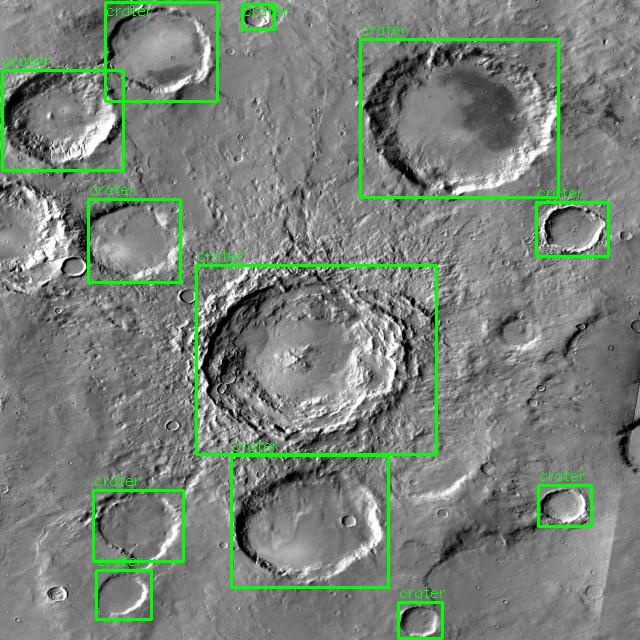
\includegraphics[width=0.75\textwidth]
			{../1-Project-Code/ground_truth_examples/015_png.rf.7d5b2091b6339c9480a171a59c52c3b9.jpg}
		\end{center}
		
		\begin{itemize}
			\item Bounding boxes generated from YOLO labels.
			\item Used to verify annotation quality before training.
			\item Important for ensuring consistent crater localization.
		\end{itemize}
		
	\end{frame}
	
	% -------------------------------------------------
	\section{Related Work}
	
	\begin{frame}{Related Work}
		
		\begin{itemize}
			\item Classical crater detection methods:
			\begin{itemize}
				\item edge detection,
				\item Hough transforms,
				\item template matching,
				\item morphological operations.
			\end{itemize}
			
			\vspace{0.3cm}
			
			\item Modern crater detection methods:
			\begin{itemize}
				\item CNN-based detectors,
				\item segmentation networks,
				\item YOLO architectures,
				\item transformer-based vision systems.
			\end{itemize}
			
			\vspace{0.3cm}
			
			\item Recent research trends:
			\begin{itemize}
				\item foundation models,
				\item multimodal vision systems,
				\item automated planetary terrain analysis.
			\end{itemize}
			
		\end{itemize}
		
	\end{frame}
	
	% -------------------------------------------------
	\section{Methodology}
	
	\begin{frame}{Overall Detection Pipeline}
		
		\begin{center}
			
			\fbox{Planetary Surface Images}
			
			\vspace{0.15cm}
			
			$\downarrow$
			
			\vspace{0.15cm}
			
			\fbox{Ground Truth Verification}
			
			\vspace{0.15cm}
			
			$\downarrow$
			
			\vspace{0.15cm}
			
			\fbox{YOLOv8 / Faster R-CNN / RetinaNet}
			
			\vspace{0.15cm}
			
			$\downarrow$
			
			\vspace{0.15cm}
			
			\fbox{Model Training}
			
			\vspace{0.15cm}
			
			$\downarrow$
			
			\vspace{0.15cm}
			
			\fbox{Prediction Generation}
			
			\vspace{0.15cm}
			
			$\downarrow$
			
			\vspace{0.15cm}
			
			\fbox{Evaluation and Comparison}
			
		\end{center}
		
	\end{frame}
	
	% -------------------------------------------------
	\begin{frame}{YOLOv8}
		
		\begin{columns}
			
			\column{0.55\textwidth}
			
			\begin{itemize}
				\item One-stage object detector.
				\item Simultaneous classification and localization.
				\item Lightweight and efficient architecture.
				\item Used pretrained \texttt{yolov8n.pt} weights.
				\item Trained for 50 epochs.
			\end{itemize}
			
			\column{0.4\textwidth}
			
			\begin{center}
				\fbox{Input Image}
				
				\vspace{0.2cm}
				
				$\downarrow$
				
				\vspace{0.2cm}
				
				\fbox{Feature Extraction}
				
				\vspace{0.2cm}
				
				$\downarrow$
				
				\vspace{0.2cm}
				
				\fbox{Bounding Box Prediction}
			\end{center}
			
		\end{columns}
		
	\end{frame}
	
	% -------------------------------------------------
	\begin{frame}{Faster R-CNN and RetinaNet}
		
		\begin{columns}
			
			\column{0.48\textwidth}
			
			\textbf{Faster R-CNN}
			
			\begin{itemize}
				\item Two-stage detector.
				\item Uses Region Proposal Network.
				\item Strong localization refinement.
				\item ResNet50-FPN backbone.
			\end{itemize}
			
			\column{0.48\textwidth}
			
			\textbf{RetinaNet}
			
			\begin{itemize}
				\item One-stage detector.
				\item Uses focal loss.
				\item Designed for class imbalance.
				\item ResNet50-FPN backbone.
			\end{itemize}
			
		\end{columns}
		
		\vspace{0.5cm}
		
		\begin{center}
			\fbox{Transfer Learning with Pretrained COCO Weights}
		\end{center}
		
	\end{frame}
	
	% -------------------------------------------------
	\begin{frame}{Training Configuration}
		
		\begin{table}[h]
			\centering
			\begin{tabular}{lccc}
				\toprule
				Model & Epochs & Batch Size & Framework \\
				\midrule
				YOLOv8 & 50 & 8 & Ultralytics \\
				Faster R-CNN & 3 & 2 & torchvision \\
				RetinaNet & 3 & 2 & torchvision \\
				\bottomrule
			\end{tabular}
		\end{table}
		
		\vspace{0.4cm}
		
		\begin{itemize}
			\item Transfer learning used for all models.
			\item YOLO-format crater labels converted for torchvision detectors.
			\item Evaluation metrics:
			\begin{itemize}
				\item Precision,
				\item Recall,
				\item mAP@0.5,
				\item mAP@0.5:0.95.
			\end{itemize}
		\end{itemize}
		
	\end{frame}
	
	% -------------------------------------------------
	\section{Results}
	
	\begin{frame}{Quantitative Results}
		
		\begin{table}[h]
			\centering
			\begin{tabular}{lccc}
				\toprule
				Model & mAP@0.5 & mAP@0.5:0.95 & mAP@0.75 \\
				\midrule
				YOLOv8 & 0.700 & 0.366 & 0.374 \\
				Faster R-CNN & 0.691 & 0.354 & 0.314 \\
				RetinaNet & 0.002 & 0.001 & 0.000 \\
				\bottomrule
			\end{tabular}
		\end{table}
		
		\vspace{0.4cm}
		
		\begin{itemize}
			\item YOLOv8 achieved strongest overall performance.
			\item Faster R-CNN achieved competitive localization.
			\item RetinaNet struggled under limited-data conditions.
		\end{itemize}
		
	\end{frame}
	
	% -------------------------------------------------
	\begin{frame}{Training Curves}
		
		\begin{center}
			
\includegraphics[width=0.9\textwidth]
			{../1-Project-Code/runs/detect/crater_detector/results.png}
		\end{center}
		
		\begin{itemize}
			\item Stable convergence observed during YOLOv8 training.
			\item Validation metrics improved progressively.
		\end{itemize}
		
	\end{frame}
	
	% -------------------------------------------------
	\begin{frame}{Precision-Recall Curve}
		
		\begin{center}
			\includegraphics[width=0.8\textwidth]
			{../1-Project-Code/runs/detect/crater_detector/BoxPR_curve.png}
		\end{center}
		
		\begin{itemize}
			\item Strong precision-recall behavior.
			\item Detector maintained relatively low false-positive rate.
		\end{itemize}
		
	\end{frame}
	
	% -------------------------------------------------
	\begin{frame}{F1 Curve and Confusion Matrix}
		
		\begin{columns}
			
			\column{0.48\textwidth}
			
			\includegraphics[width=\textwidth]
			{../1-Project-Code/runs/detect/crater_detector/BoxF1_curve.png}
			
			\column{0.48\textwidth}
			
			\includegraphics[width=\textwidth]
			{../1-Project-Code/runs/detect/crater_detector/confusion_matrix_normalized.png}
			
		\end{columns}
		
		\vspace{0.3cm}
		
		\begin{itemize}
			\item Strong crater classification capability.
			\item Balanced precision and recall behavior.
		\end{itemize}
		
	\end{frame}
	
	% -------------------------------------------------
	\begin{frame}{Qualitative Detection Results}
		
		\begin{columns}
			
			\column{0.48\textwidth}
			
			\textbf{Ground Truth}
			
			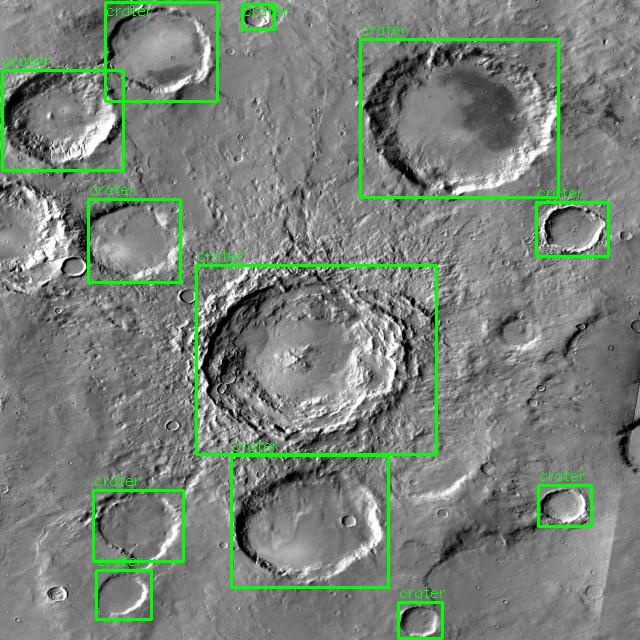
\includegraphics[width=\textwidth]
			{../1-Project-Code/ground_truth_examples/015_png.rf.7d5b2091b6339c9480a171a59c52c3b9.jpg}
			
			\column{0.48\textwidth}
			
			\textbf{YOLOv8 Predictions}
			
			
\includegraphics[width=\textwidth]
			{../1-Project-Code/runs/detect/crater_test_predictions/015_png.rf.7d5b2091b6339c9480a171a59c52c3b9.jpg}
			
		\end{columns}
		
	\end{frame}
	
	% -------------------------------------------------
	\begin{frame}{Detector Output Comparison}
		\centering
		\scriptsize
		
		\begin{tabular}{cc}
			\textbf{Ground Truth} & \textbf{YOLOv8} \\[-0.05cm]
			
			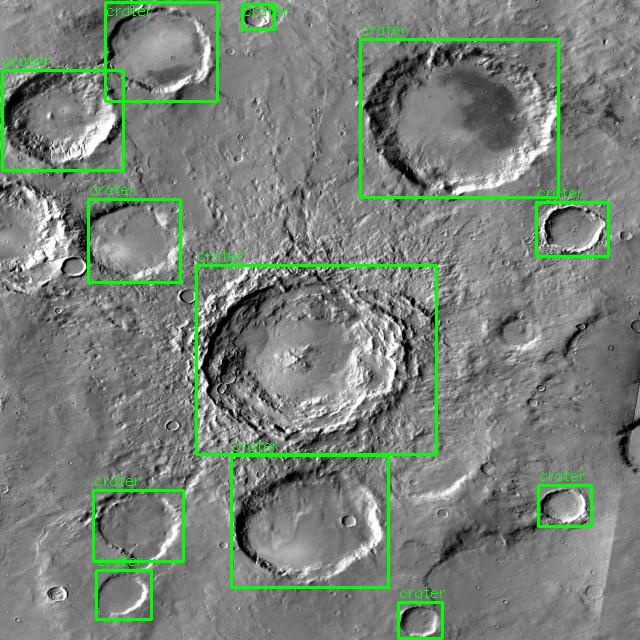
\includegraphics[width=0.31\textwidth]
			{../1-Project-Code/ground_truth_examples/015_png.rf.7d5b2091b6339c9480a171a59c52c3b9.jpg}
			&
			
\includegraphics[width=0.31\textwidth]
			{../1-Project-Code/runs/detect/crater_test_predictions/015_png.rf.7d5b2091b6339c9480a171a59c52c3b9.jpg}
			\\[-0.05cm]
			
			\textbf{Faster R-CNN} & \textbf{RetinaNet} \\[-0.05cm]
			
			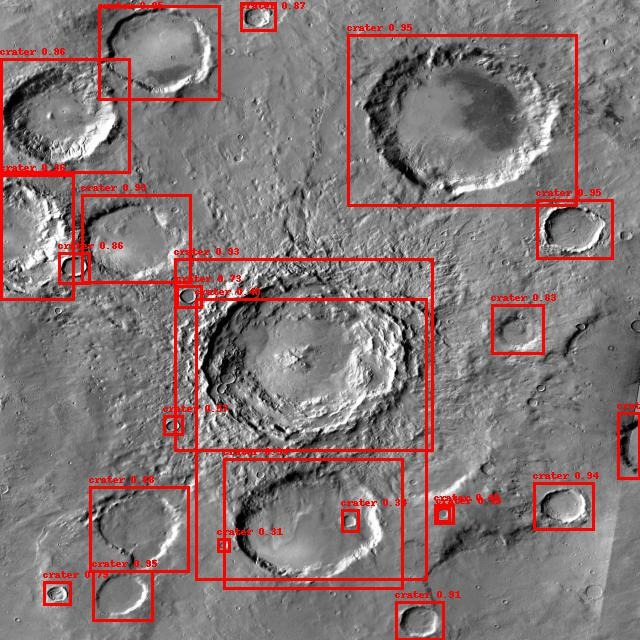
\includegraphics[width=0.31\textwidth]
			{../1-Project-Code/torchvision_predictions/faster_rcnn_prediction_015.jpg}
			&
			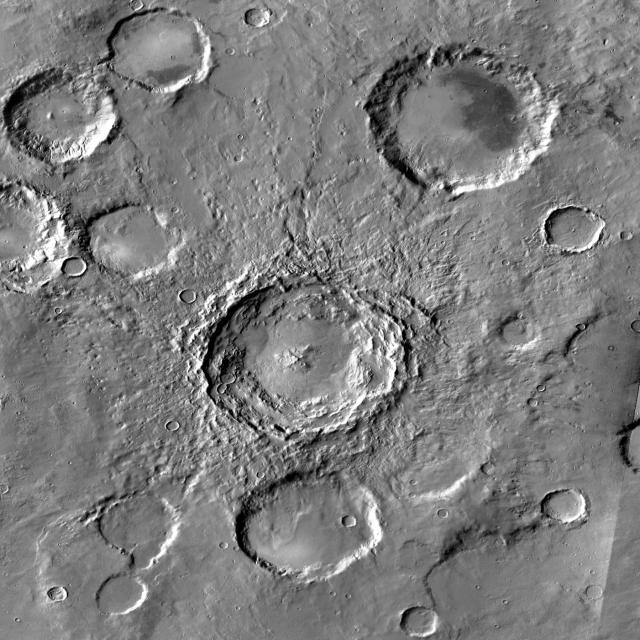
\includegraphics[width=0.31\textwidth]
			{../1-Project-Code/torchvision_predictions/retinanet_prediction_015.jpg}
		\end{tabular}
		
		\vspace{0.08cm}
		
		\scriptsize RetinaNet produced no confident detections at threshold 0.3.
		
	\end{frame}
	
	% -------------------------------------------------
	\begin{frame}{Final Model Comparison}
		
		\begin{center}
			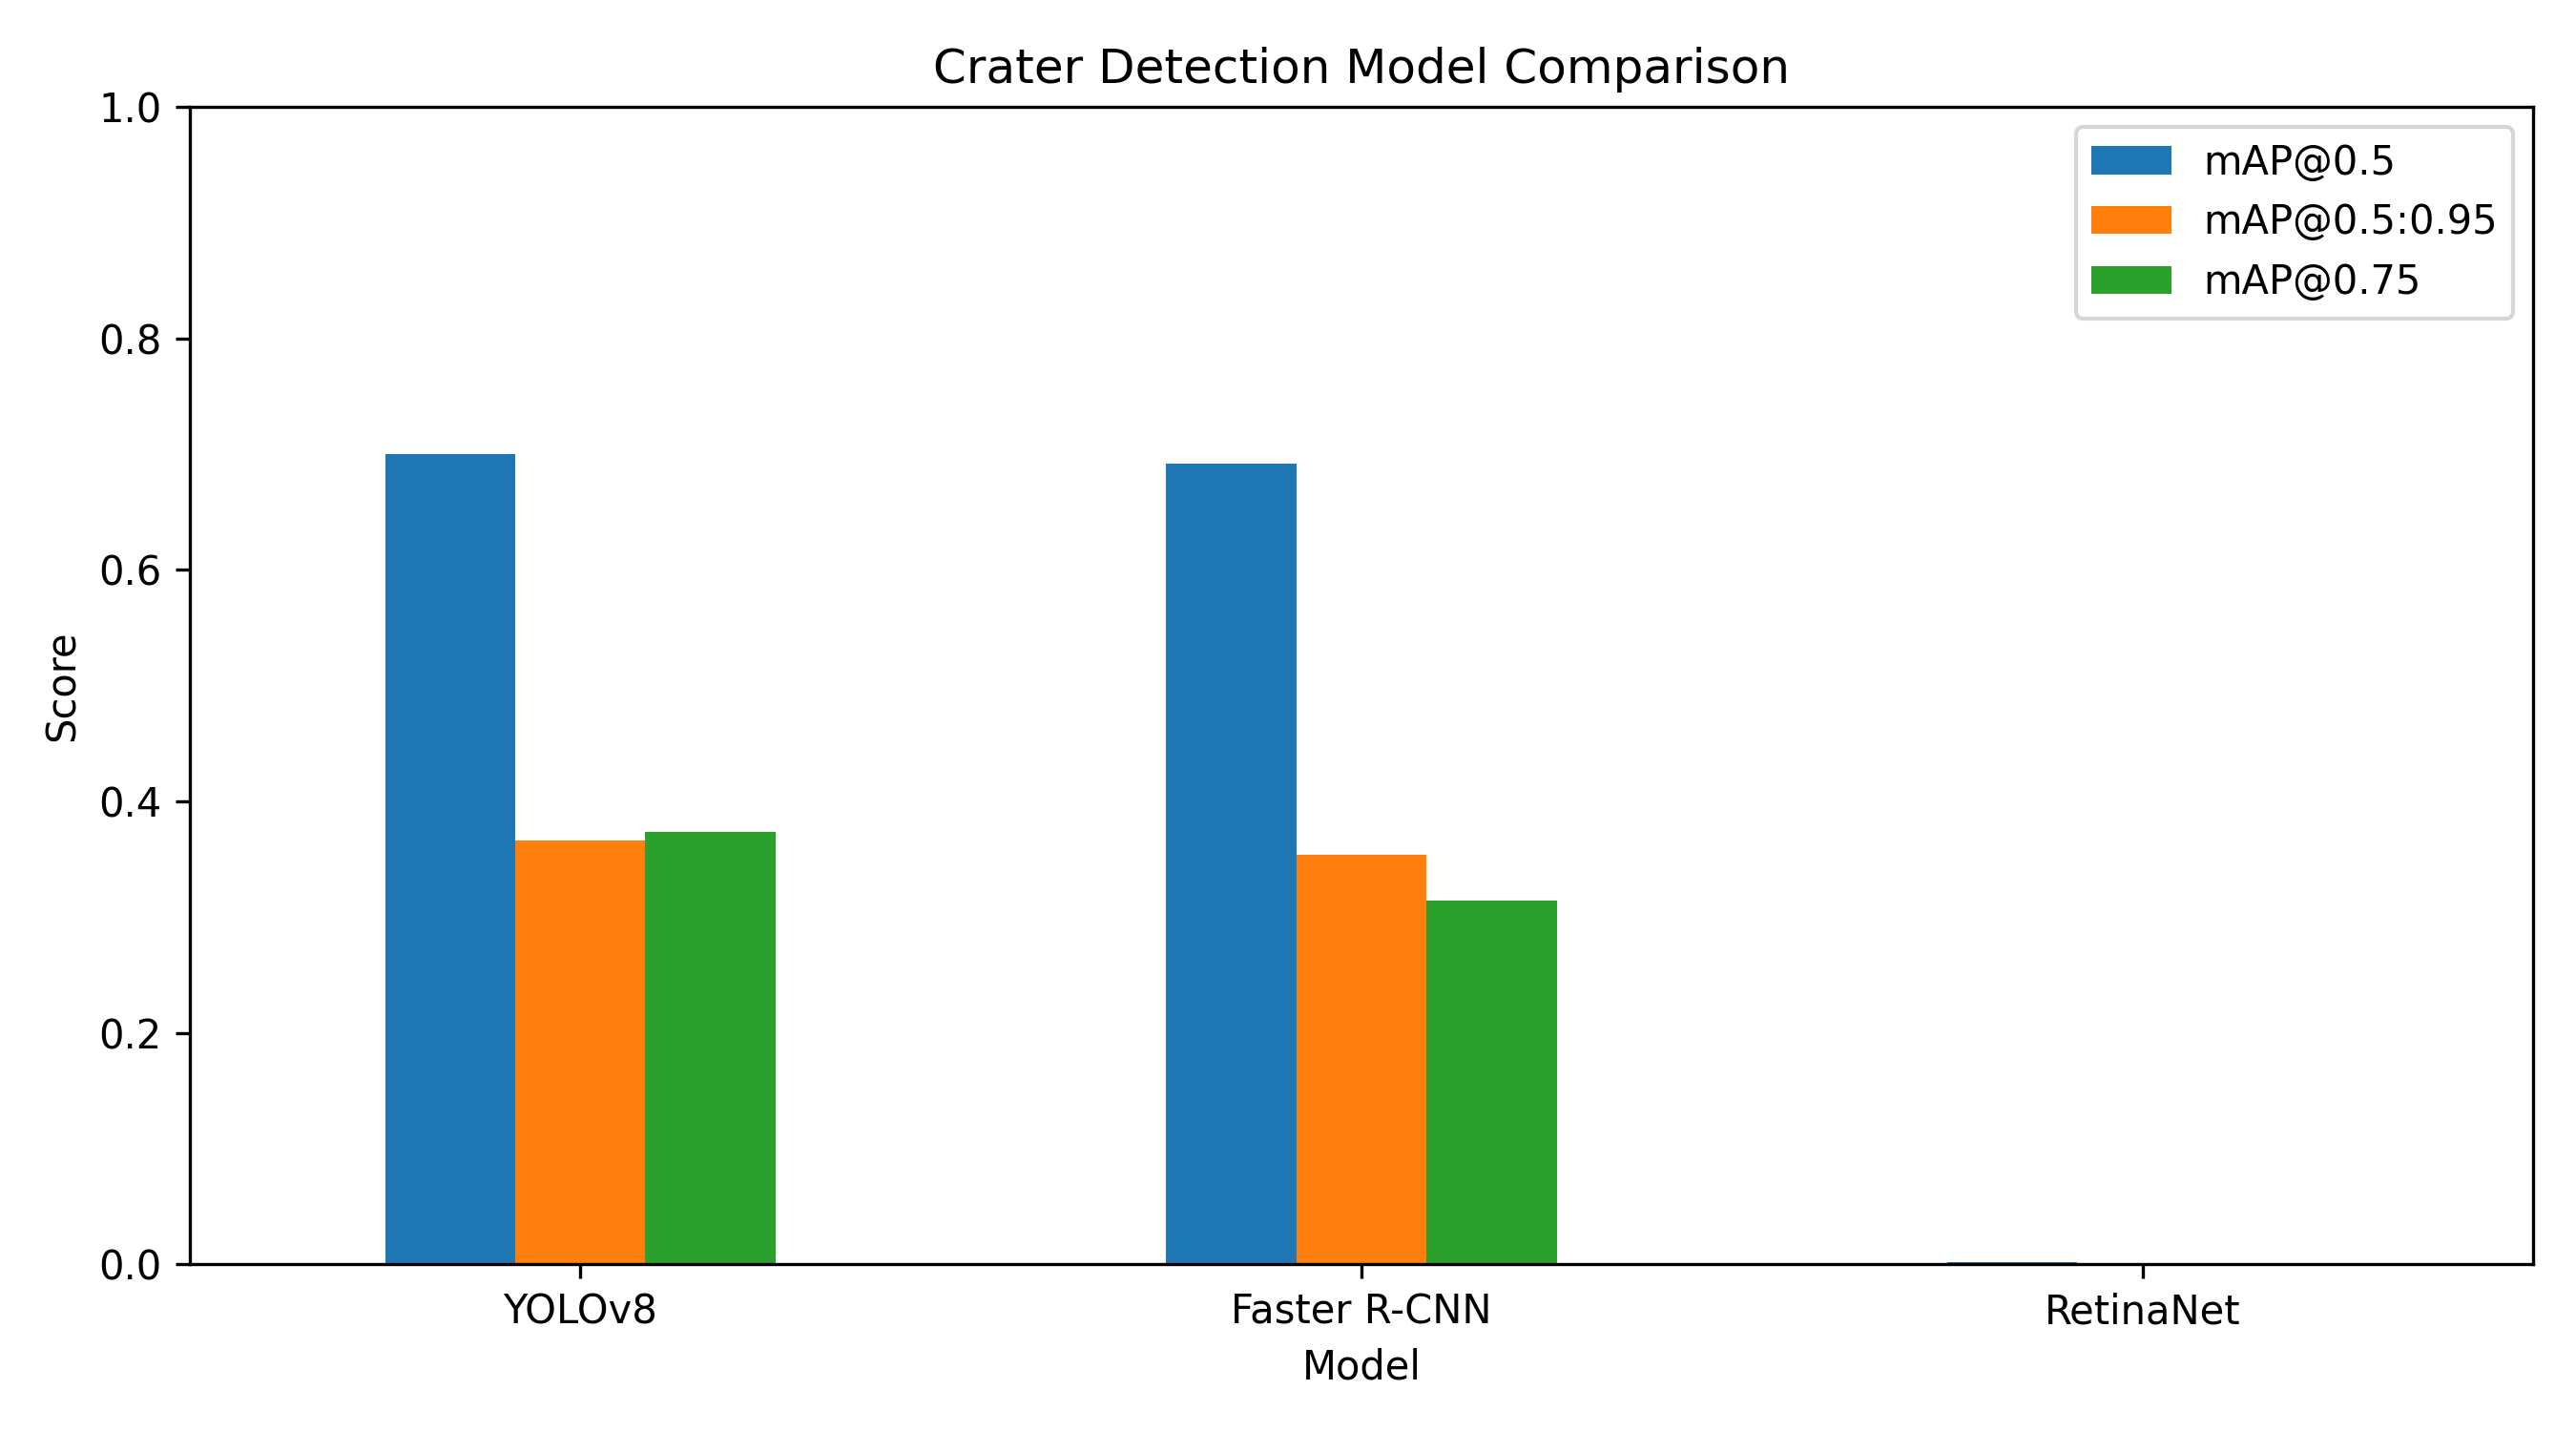
\includegraphics[width=0.85\textwidth]
			{../1-Project-Code/model_comparison_plot.png}
		\end{center}
		
		\begin{itemize}
			\item YOLOv8 achieved strongest crater localization.
			\item Faster R-CNN achieved similar performance.
			\item RetinaNet underperformed due to limited-data training.
		\end{itemize}
		
	\end{frame}
	
	% -------------------------------------------------
	\section{Discussion}
	
	\begin{frame}{Discussion}
		
		\begin{itemize}
			\item YOLOv8 achieved strongest overall performance.
			\item One-stage architecture provided efficient detection.
			\item Faster R-CNN demonstrated strong localization refinement.
			\item RetinaNet struggled under limited-data conditions.
		\end{itemize}
		
		\vspace{0.4cm}
		
		\textbf{Major Crater Detection Challenges}
		
		\begin{itemize}
			\item overlapping crater structures,
			\item degraded crater rims,
			\item low-contrast terrain,
			\item varying crater scales,
			\item illumination variability.
		\end{itemize}
		
	\end{frame}
	
	% -------------------------------------------------
	\begin{frame}{Future Work}
		
		\begin{itemize}
			\item Larger crater datasets.
			\item Higher-resolution planetary imagery.
			\item Transformer-based object detectors.
			\item Foundation-model-based crater detection.
			\item Crater segmentation methods.
			\item Semi-supervised learning.
			\item Multi-class geological feature detection.
		\end{itemize}
		
		\vspace{0.5cm}
		
		\begin{center}
			\fbox{Future Direction: Foundation Models + Planetary Vision Systems}
		\end{center}
		
	\end{frame}
	
	% -------------------------------------------------
	\section{Conclusion}
	
	\begin{frame}{Conclusion}
		
		\begin{itemize}
			\item Developed a complete crater detection pipeline.
			\item Verified and visualized YOLO-format ground truth.
			\item Trained and compared multiple deep learning detectors.
			\item YOLOv8 achieved best overall crater detection performance.
			\item Demonstrated feasibility of deep learning for planetary terrain analysis.
		\end{itemize}
		
		\vspace{0.6cm}
		
		\begin{center}
			\Large
			Thank You
		\end{center}
		
	\end{frame}
	
	% -------------------------------------------------
	\begin{frame}{References}
		
		\footnotesize
		
		\begin{thebibliography}{99}
			
			\bibitem{yolo}
			J. Redmon et al.,
			``You Only Look Once: Unified, Real-Time Object Detection,''
			CVPR, 2016.
			
			\bibitem{fasterrcnn}
			S. Ren et al.,
			``Faster R-CNN: Towards Real-Time Object Detection with Region Proposal Networks,''
			IEEE TPAMI, 2017.
			
			\bibitem{retinanet}
			T.-Y. Lin et al.,
			``Focal Loss for Dense Object Detection,''
			ICCV, 2017.
			
			\bibitem{ultralytics}
			Ultralytics,
			``YOLOv8 Documentation,''
			https://docs.ultralytics.com
			
			\bibitem{pytorch}
			PyTorch,
			``Torchvision Object Detection Models,''
			https://pytorch.org/vision/stable/models.html
			
		\end{thebibliography}
		
	\end{frame}
	
	% -------------------------------------------------
\end{document}
```
